\documentclass[11pt]{article}

\usepackage[a4paper,margin=2.4cm]{geometry}
\usepackage{amsmath,amssymb}
\usepackage{booktabs}
\usepackage{siunitx}
\usepackage{graphicx}
\usepackage{xcolor}
\usepackage[hidelinks]{hyperref}
\usepackage{enumitem}

\newcommand{\bplus}{\beta^{+}}
\newcommand{\Cl}[1]{{}^{#1}\mathrm{C}}
\newcommand{\Ox}[1]{{}^{#1}\mathrm{O}}
\newcommand{\Nt}[1]{{}^{#1}\mathrm{N}}
\newcommand{\Rd}{R_{\mathrm d}}
\newcommand{\Rp}{R_{\mathrm p}}


\title{Generating the positron-emitter source for proton-therapy PET using \texttt{ptcryspg4}}
\author{J.J. G\'omez-Cadenas\\\texttt{jjgomezcadenas@gmail.com}}
\date{Documentation last rebuild: \today}

\begin{document}
\maketitle

\begin{abstract}
The package \texttt{ptcryspg4} simulates a proton beam stopping in a phantom,
records where positron emitters are created and where their positrons annihilate,
producing gamma pairs that can be detected by a PET scanner. The software defines a set of phantoms (currently a simple cylinder, an uniform ``head'' phantom and an MIRD ``head'' phantom are implemented), runs a Geant4 simulation of the proton beam traversing the phantom and outputs a set of CSV files that describe the resulting annihilation source (e.g., the trail of 2-$\gamma$ emissions that follows the proton beam) and the normalisation to a given (specified dose).  The result product is a ``scenario'' (phantom, beam, dose and the resulting output) that can be read out by a downstream PET simulation. 
\end{abstract}

\section{Tracking proton dose with \texorpdfstring{$\bplus$}{beta+}}
\label{sec:physics-intro}

Conventional, photon-based radiation therapy deposits a high dose where the beam enters the patient, weakening gradually as it traverses tissue. A proton beam instead releases most of its energy near the end of its track, at the so-called Bragg peak; combining protons of several energies produces a spread-out Bragg peak (SOBP). The proton entrance dose is therefore much lower and no dose is deposited beyond the target volume. This lets proton therapy shape the high-dose region to the three-dimensional outline of the target while sparing the surrounding tissue, making it preferable for tumours with irregular shapes or close to critical structures. Its integral dose is also much smaller, about 60\% below that of photon therapy, which favours its use in paediatric patients, where the risk of a secondary tumour induced by dose to normal tissue is a concern \cite{parodi2023, 
parodi2024}.

The steep dose fall-off at the Bragg peak makes planning uncertainties more consequential than in photon therapy. A range error can leave part of a tumour with no dose at all (under-shooting), or deliver a full dose to the normal tissue lying distal to the beam (over-shooting). Verification is therefore of utmost importance, both to exploit the technique and to assess treatment-planning safety margins. Since proton beams stop completely in the body, direct in vivo monitoring is difficult, and at present the only practical approach is PET imaging of the proton-induced positron emitters.

During irradiation, positron emitters are produced along the beam path through nuclear fragmentation, leaving a radiotracer footprint that a PET scanner can image. In soft tissue the main species are $^{11}$C, $^{13}$N and $^{15}$O. The last dominates right after irradiation, owing to the high oxygen density of tissue, but its short half-life (about 2 minutes) means $^{11}$C takes over after a few minutes\cite{zhu2013proton}.

Dose deposition and positron-emitter production are distinct processes: dose is deposited electromagnetically, by ionising and exciting atomic electrons, whereas emitter production proceeds through nuclear reactions whose yield depends on proton fluence, energy-dependent reaction cross sections and target-nuclei density. The PET activity distribution is thus quite different from the dose distribution, with almost no activity in the $\sim$1~cm before the Bragg peak, owing to nuclear reaction thresholds; the measured activity must therefore be compared with a predicted distribution.

\subsection{Induced activity and its time evolution}
\label{sec:activity}

Protons traversing biological tissue undergo nuclear reactions, such as for example,
$p + \Ox{16} \rightarrow \Ox{15} + n + p$, followed by 
$\Ox{15} \rightarrow \Nt{15} + \beta^+ + \nu_e$ ($T_{1/2} = 122 s \approx\SI{2}{min}$). 
Other relevant $\beta^+$ emitters are $\Cl{11}$ ($T_{1/2}\approx\SI{20}{min}$), $\Nt{13}$ ($T_{1/2}\approx\SI{10}{min}$),
and the shorter-lived $\Ox{14}$ ($T_{1/2}=\SI{70.6}{s}$) and $\Cl{10}$
($T_{1/2}=\SI{19.3}{s}$)~\cite{zhu2013proton,parodi2008comparison}. Because the
signal is a mixture of species with very different half-lives, the measurement
depends strongly on when the scanner acquires.

\begin{figure}[htbp]
\centering
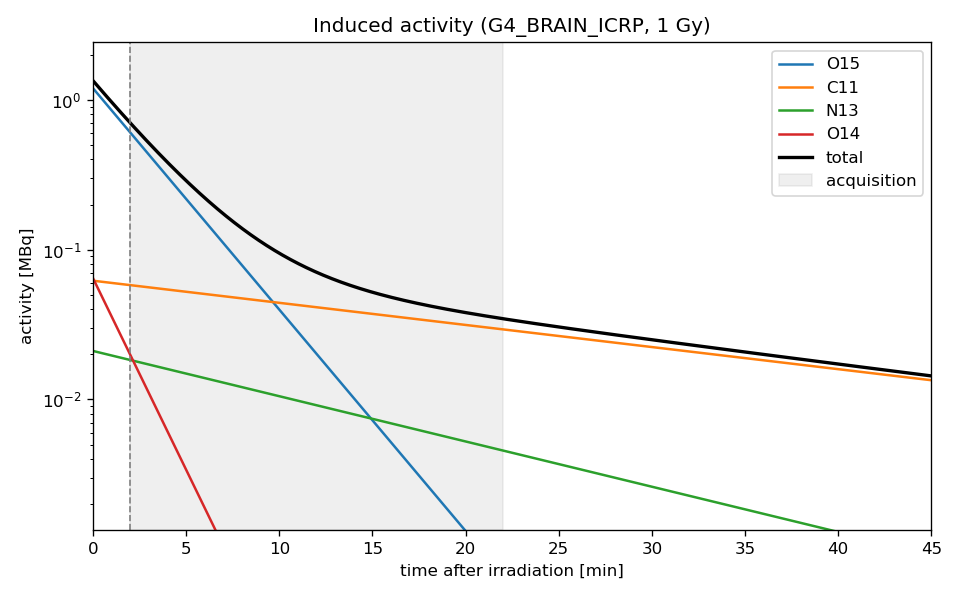
\includegraphics[width=0.8\linewidth]{activity.png}
\caption{Activity of the main positron-emitting species as a function of time after
irradiation, from a Geant4 simulation of a \SI{1}{Gy} proton field in an ICRP
brain-tissue phantom. The shaded band marks a representative in-room acquisition
window. The shortest-lived emitter, $\Cl{10}$ ($T_{1/2}=\SI{19.3}{s}$), has
effectively vanished before the window opens and is not drawn.}
\label{fig:activity}
\end{figure}

Figure~\ref{fig:activity} shows the activity by species from a Geant4 simulation of
a \SI{1}{Gy} proton field in an ICRP brain-tissue phantom.
The total peaks at $\sim$\SI{1.34}{MBq} at the end of the beam, dominated by
$\Ox{15}$ at $\sim$\SI{1.2}{MBq}. But $\Ox{15}$ decays with a \SI{2}{min} half-life:
by \SI{10}{min} it has fallen to the level of $\Cl{11}$, and by $\sim$\SI{15}{min}
it has effectively gone. The very short-lived emitters disappear even sooner ---
$\Cl{10}$ within about a minute, $\Ox{14}$ within a few. The $\Cl{11}$ component is
nearly flat ($T_{1/2}\approx\SI{20}{min}$) at $\sim$\SI{0.06}{MBq} and comes to
dominate after $\sim$\SIrange{10}{13}{min}.

Two consequences follow from this decay pattern. First, the scan must start as soon as possible after the beam stops, since an in-beam scan can be impractical because of backgrounds. Second, every photon pair is precious. These two requirements are somewhat contradictory. An immediate scan requires an in-line PET, which must let the beam through; the resulting open geometry has poor geometrical acceptance. The opposite approach, moving the patient to an off-room PET, is also impractical: after about five minutes the activity has fallen sharply, through both isotope decay and biological washout. An in-room PET --- a full-ring scanner in the treatment room --- is an affordable compromise. An in-room scan at $\sim$\SI{2}{min} still sees $\sim$\SI{0.7}{MBq}, with $\Ox{15}$ still dominant; an offline scan at $\geq$\SI{15}{min} sees only $\sim$\SI{0.04}{MBq}, essentially $\Cl{11}$ alone --- more than an order of magnitude less signal.
%Since
%$\Ox{15}$ also has the longest positron range, the in-room case is both the
%brightest and the one where the positron-range blur matters most.

\subsection{Decay kinetics and the measured counts}
\label{sec:kinetics}

Each species $j$ decays with constant $\lambda_j=\ln 2/T_{1/2,j}$ (assumed
$100\%$ $\bplus$). Take a delivery of duration $t_{\mathrm{irr}}$ at an
approximately constant production rate, a delay $t_{\mathrm{del}}$ before the scan
starts, and an acquisition window of length $t_{\mathrm{meas}}$. For a continuous
(cyclotron-like) delivery, the number of decays of species $j$ collected inside the
window~\cite{parodi2008comparison} is
\begin{equation}
N_{j,\mathrm{meas}} =
P_j \,
\underbrace{\frac{1-e^{-\lambda_j t_{\mathrm{irr}}}}{\lambda_j t_{\mathrm{irr}}}}_{\text{undecayed at end of beam}}
\;
\underbrace{e^{-\lambda_j t_{\mathrm{del}}}}_{\text{survive the delay}}
\;
\underbrace{\left(1-e^{-\lambda_j t_{\mathrm{meas}}}\right)}_{\text{decay in the window}} ,
\label{eq:nmeas}
\end{equation}
where $P_j$ is the integral production of species $j$ over the whole field (the
number of nuclei created), which is proportional to the delivered dose. The three
factors read left to right:
\begin{itemize}[nosep]
\item $\dfrac{1-e^{-\lambda_j t_{\mathrm{irr}}}}{\lambda_j t_{\mathrm{irr}}}$ --- the
fraction still undecayed at the end of the beam. It accounts for production and decay
happening at the same time during irradiation; it tends to $1$ for long-lived species
($\lambda_j t_{\mathrm{irr}}\ll 1$) and is smaller for short-lived ones.
\item $e^{-\lambda_j t_{\mathrm{del}}}$ --- decay during the delay between the end of
the beam and the start of acquisition.
\item $1-e^{-\lambda_j t_{\mathrm{meas}}}$ --- the fraction of the survivors that
decay while the scanner is acquiring.
\end{itemize}
The full derivation, including pulsed (synchrotron) deliveries, is in
\texttt{03\_decay\_kinetics.tex}. 
%Equation~\eqref{eq:nmeas} is exactly what turns the
%\emph{produced} emitters of the proton run into the \emph{measured} counts; it is
%applied in Sec.~\ref{sec:handoff}.

\subsection{$\beta^+$ Activity vs proton dose}
\label{sec:source-picture}

\begin{figure}[htbp]
\centering
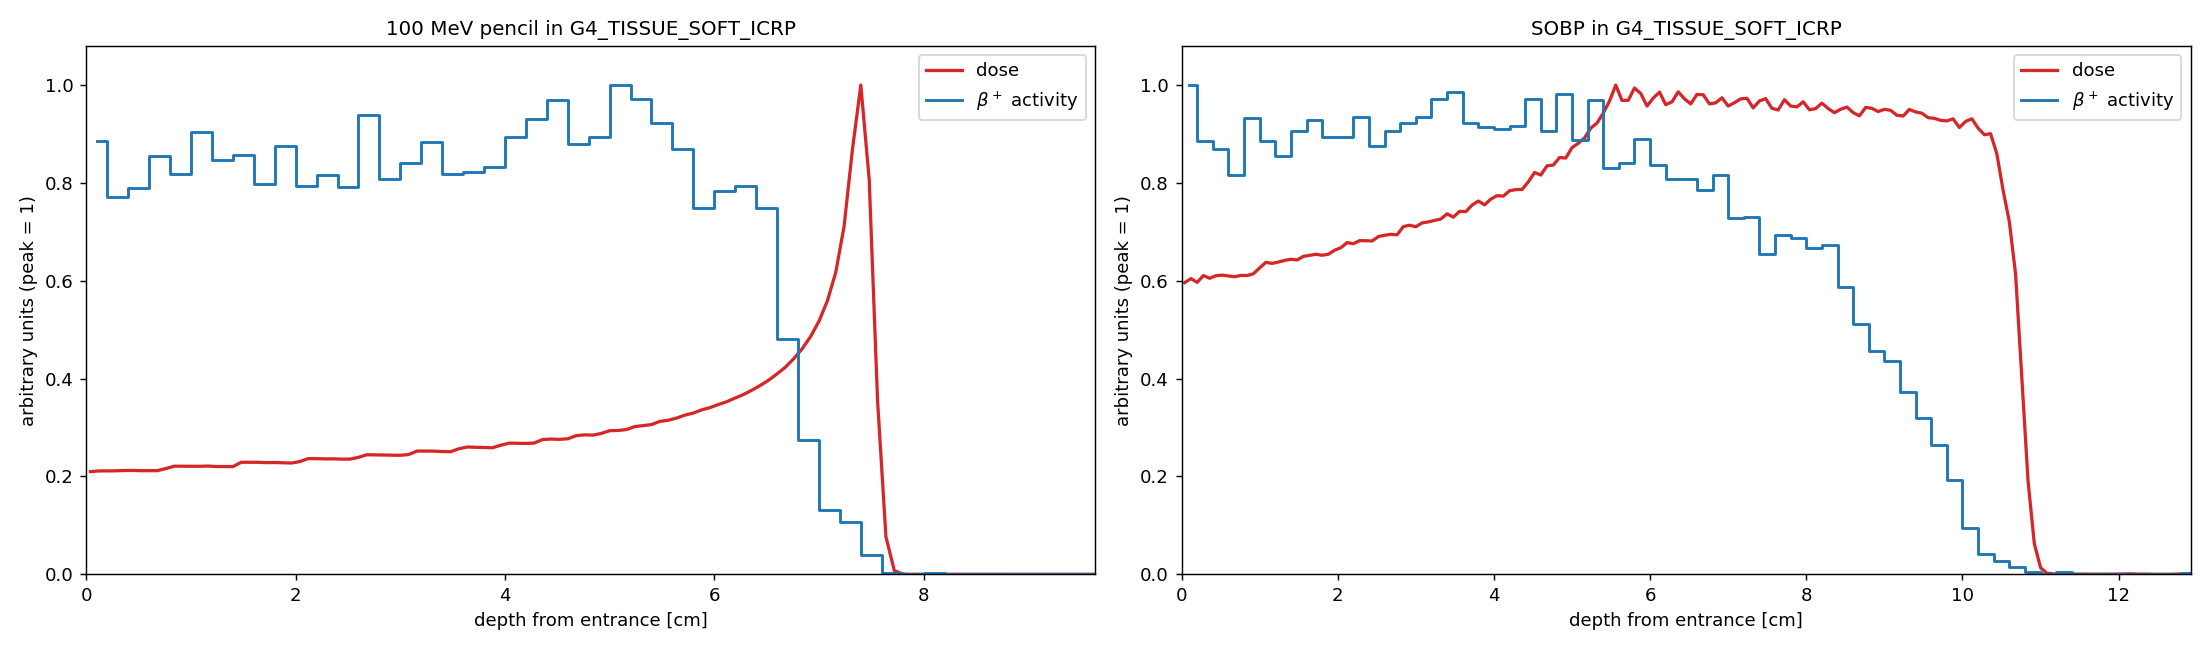
\includegraphics[width=\linewidth]{dose_activity.png}
\caption{Dose (red) and total $\bplus$ activity (blue), in arbitrary units (each
curve normalised to its own peak), for two beams in the same soft-tissue cylinder.
\emph{Left:} a \SI{100}{MeV} pencil --- a single Bragg peak. \emph{Right:} a
spread-out Bragg peak (SOBP), several energies combined into a flat dose plateau
across a target at \SIrange{5.5}{10.5}{cm} depth. In both cases the $\bplus$
activity is roughly flat along the proton track and falls to zero just before the
distal dose edge; that fall-off, $A(x)\to 0$, marks the beam's distal reach.}
\label{fig:source}
\end{figure}


%\begin{figure}[htbp]
%\centering
%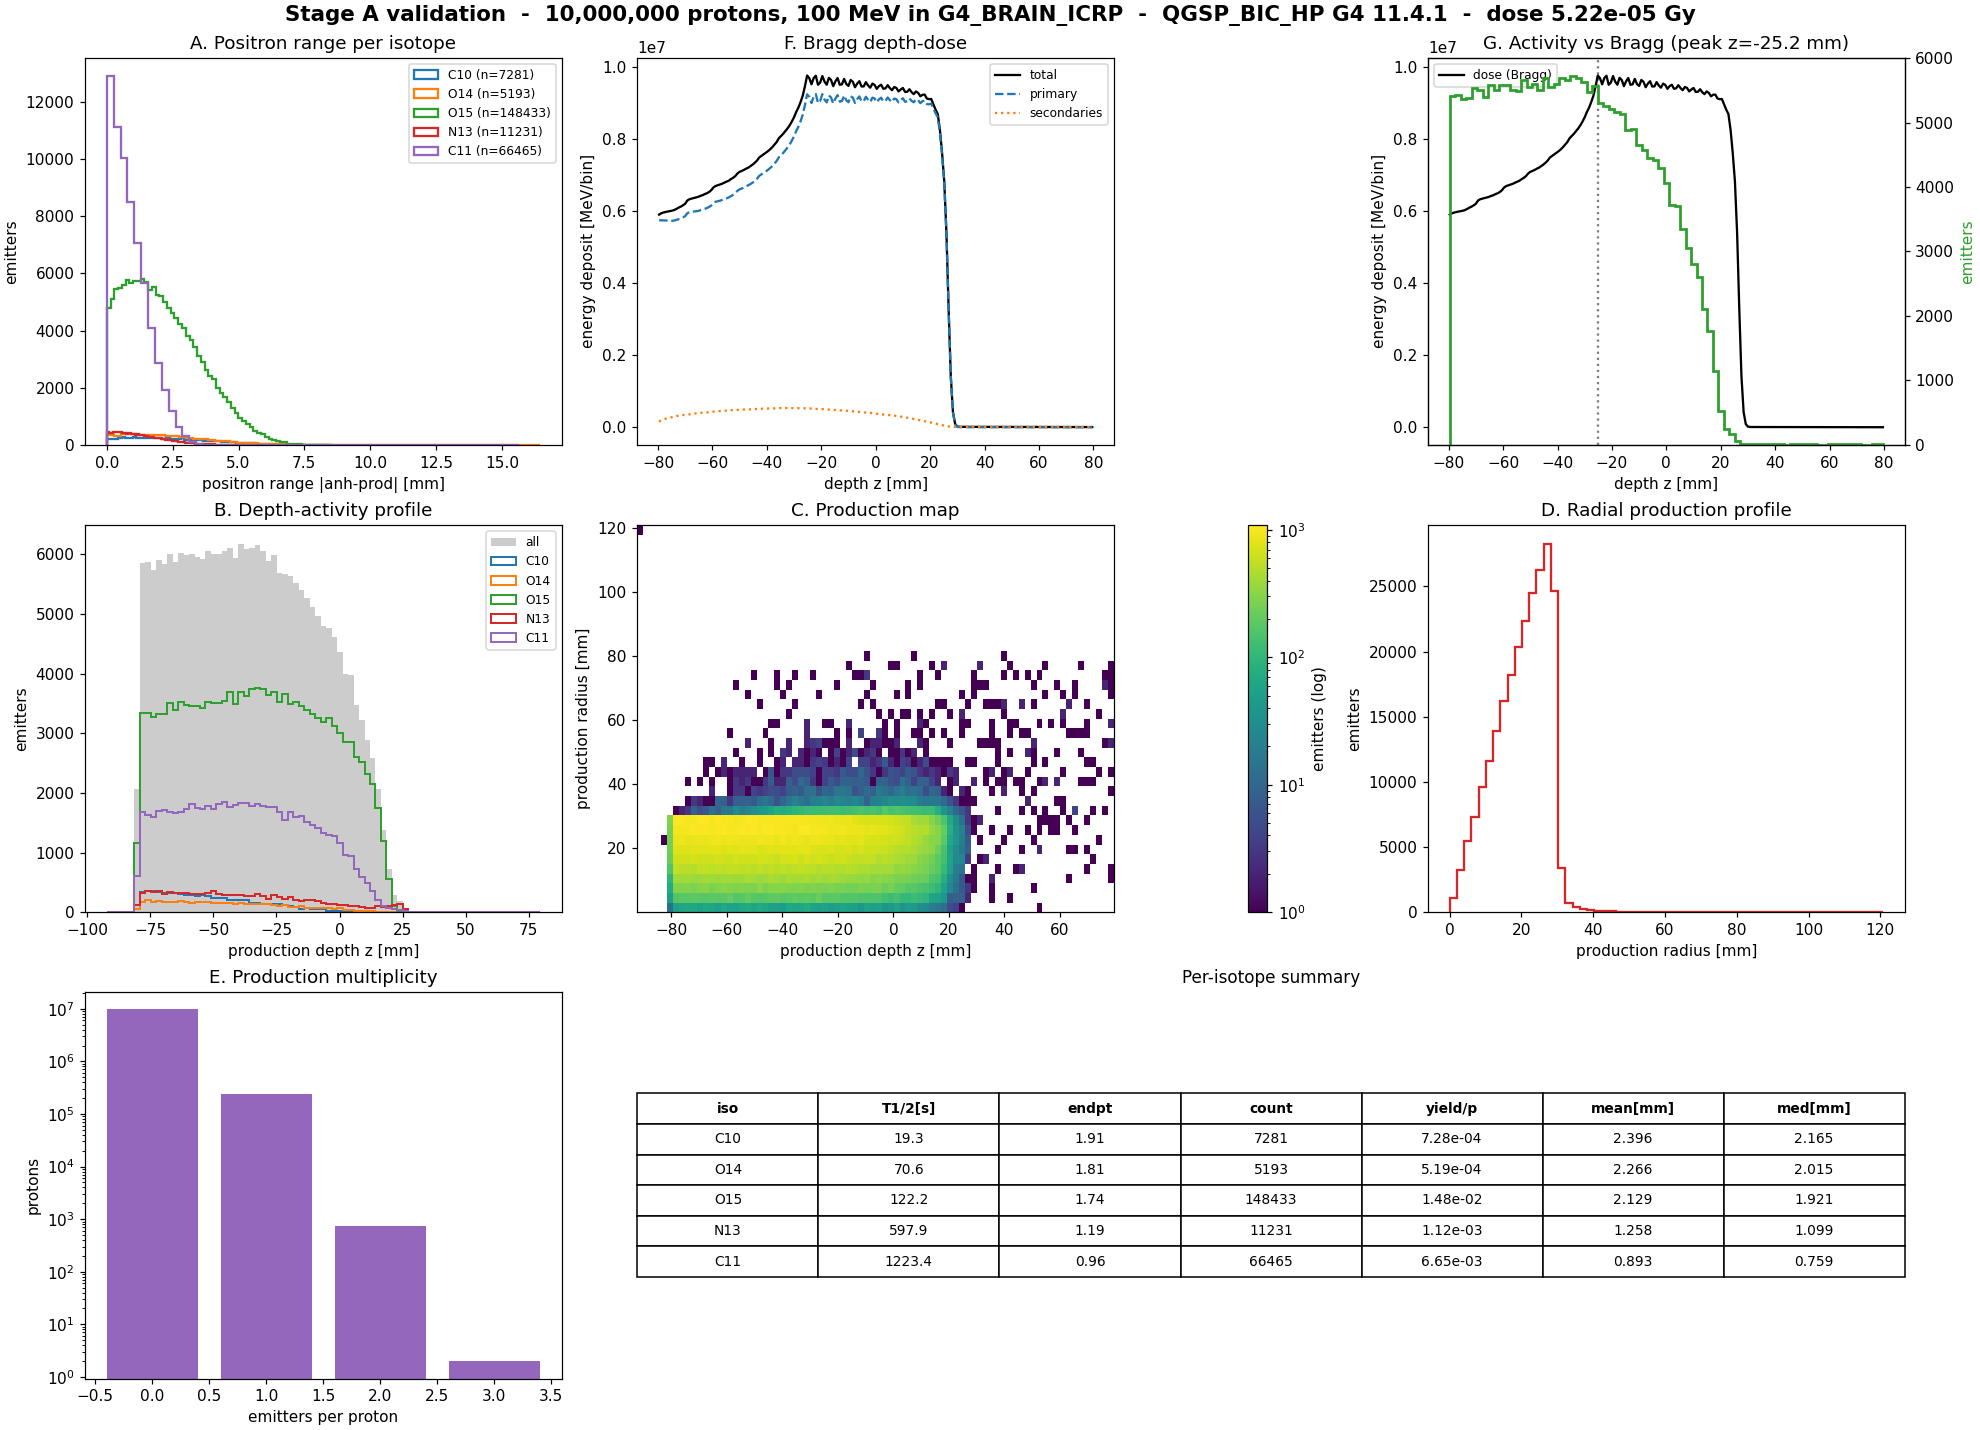
\includegraphics[width=\linewidth]{transport_validation.png}
%\caption{The generated source, from a \SI{1}{Gy} SOBP field in the brain phantom
%(\texttt{analysis\_transport/validate\_transport.py}). The panels show, among other
%diagnostics, the production map along the beam (where the activity is created,
%peaking just before the Bragg peak), the per-species spatial distributions, the
%positron-range distributions per isotope (the physical resolution floor, largest for
%$\Ox{15}$), and the depth--dose Bragg curve. This is the detector-independent source
%the pipeline hands downstream.}
%\label{fig:source}
%\end{figure}

The left panel of Figure~\ref{fig:source} shows a pencil beam depositing a dose $D$ in biological tissue. The sharp Bragg peak defines the maximum of dose deposition. The figure also shows the total $\beta^+$ activity, which would correspond to an ideal PET measurement starting acquisition immediately after the beam stops.

The activity curve and the dose behave differently. As the proton beam propagates through the tissue, before the target region (and the Bragg peak), the dose is low and slowly rising, and the $\beta^+$ activity is relatively flat. At the Bragg peak the beam quickly loses energy, quenching the nuclear reactions, so the $\beta^+$ activity drops just where the Bragg ionisation rises and reaches zero in the trailing edge of the peak. Formally, if $A(x)$ is the activity along the beam line, the distal reach of the beam is estimated by the point $x'$ at which $A(x')=0$.

The right panel of Figure~\ref{fig:source} shows the same comparison for a spread-out Bragg peak --- the field used in treatment, where several proton energies combine to deliver a flat dose plateau across the target volume. The same reasoning holds: the $\beta^+$ activity is roughly flat across the plateau and falls to zero just past its distal edge, so $A(x) \rightarrow 0$ marks the distal edge of the target volume.

Several real-life complications must be added to this simple picture. First, a PET scanner does not directly measure activity, only pairs of gammas; the activity must be reconstructed from the data, a non-trivial task. Second, a scanner records only a fraction of the produced gamma pairs, once geometrical and detector efficiency are folded in. Finally, the $\beta^+$ reach --- the distance a positron travels before annihilation --- introduces a genuine physical uncertainty in the determination of the distal edge of the beam.

The example just described is also idealised: a cylinder filled with biological tissue. In practice the proton beam propagates through a heterogeneous medium, which complicates the picture further.


\section{Simulating the \texorpdfstring{$\bplus$}{beta+} trail in \texttt{ptcryspg4}}
\label{sec:pipeline}

The approach is to run a Geant4 simulation of a proton beam stopping in a phantom, recording the trail of positron emitters it leaves along the way. Two ingredients define
the run:

\begin{itemize}[nosep]
\item \textbf{A beam} --- protons; either a simple pencil beam or the more realistic SOBP (Spread-Out Bragg Peak) case.
\item \textbf{A phantom} --- a body of material that stands in for the region being
treated, chosen to represent the clinical problem. Currently, \texttt{ptcryspg4} implements a homogeneous brain-tissue cylinder (used for the examples above), a homogeneous head filled with brain tissue, and a MIRD head built from three different materials (scalp, bone and brain tissue).
\end{itemize}

The code performs two steps:
\begin{enumerate}[nosep]
\item \textbf{Propagation and production --- in space.} Geant4 transports the protons
and records where each positron emitter is produced and where its positron
annihilates.
\item \textbf{Lifetime.} An analytic step folds in the radioactive
half-lives and the scanner's acquisition timing (Sec.~\ref{sec:kinetics}), computing for each emission point the number of decays that corresponds to a given dose. This second step is the handoff.
\end{enumerate}

The handoff takes the (scanner-independent) source produced by
Geant4 and applies ion decay and timing, preparing the count budget for a subsequent detector study.  The result is frozen as a {\em scenario}.

\begin{center}
\fbox{\parbox{0.95\textwidth}{\ttfamily\small
\textbf{proton run (Geant4)} \hfill \textit{runs once}\\
\hspace*{1em}protons $\to$ phantom $\to$ $\bplus$ emitter produced $\to$ positron annihilates\\
\hspace*{1em}$\Rightarrow$ emitters.csv (production + annihilation points) + run\_meta.csv\\[2pt]
\textbf{handoff (Python)}\\
\hspace*{1em}produced emitters $\to$ decay + acquisition window $\to$ measured count\\
\hspace*{1em}$\Rightarrow$ sampling\_budget\_<scenario>.csv (decays per isotope)\\[2pt]
\hspace*{1em}frozen as a named scenario; a detector simulation reads it
}}
\end{center}

\noindent The next two sections give the details of each part: the proton run
(Sec.~\ref{sec:transport}) and the handoff (Sec.~\ref{sec:handoff}).

\section{Step 1 --- the proton run (Geant4)}
\label{sec:transport}

\subsection{The beam}
\label{sec:beam}

\subsection{Mono energetic proton beam}
\label{sec:pristine}

A mono-energetic proton of energy $E$ stops at a well-defined depth, its
\textbf{range} $R$. To good approximation the two are related by the
Bortfeld power law~\cite{bortfeld1996},
\begin{equation}
R(E) = \alpha\,E^{\,p},
\label{eq:range}
\end{equation}
with, in water, $\alpha=\SI{2.2e-3}{cm\,MeV^{-p}}$ and $p=1.77$. For another
homogeneous material we scale the range by the (mass) stopping-power ratio,
which to first order is the inverse mass-density ratio,
$R_{\mathrm{mat}}\simeq R_{\mathrm{water}}/\rho_{\mathrm{rel}}$
($\rho_{\mathrm{rel}}\approx1.04$ for brain). The energy needed to reach a depth
$R$ is the inverse of Eq.~\eqref{eq:range}, $E(R)=(R/\alpha)^{1/p}$.

Equation~\eqref{eq:range} is used  to choose the \emph{layer energies}.
% the
%actual peak shapes come from Geant4, and the plateau is verified there
%(Sec.~\ref{sec:verify}), so small inaccuracies in $\alpha,p$ are corrected by
%the verification step.
In particular, one can make use that 
%A useful consequence of Eq.~\eqref{eq:range}: 
a proton that has travelled to
depth $z<R$ has residual range $R-z$ and residual energy
$\propto (R-z)^{1/p}$, so its mass stopping power (dose per unit length) scales as
\begin{equation}
S(z;R)\ \propto\ \frac{\mathrm dE}{\mathrm dz}\ \propto\ (R-z)^{\,1/p-1}.
\label{eq:stop}
\end{equation}

\subsection{SOBP as a weighted superposition}

To form a SOBP beam, one superimposes 
$N$ mono-energetic Bragg peaks at ranges $R_i$ spanning the target depth,
\begin{equation}
R_i = \Rp + \frac{i}{N-1}\,(\Rd-\Rp),\qquad i=0,\dots,N-1,
\end{equation}
($R_0=\Rp$ proximal, $R_{N-1}=\Rd$ distal), with relative fluence weights
$w_i\ge0$. The total depth--dose is their superposition,
\begin{equation}
D_{\mathrm{SOBP}}(z)=\sum_{i\,:\,R_i\ge z} w_i\,S(z;R_i).
\label{eq:super}
\end{equation}
%The gun realises Eq.~\eqref{eq:super} stochastically: each primary proton is
%assigned to layer $i$ with probability $\propto w_i$ and given energy
%$E_i=E(R_i)$.


\subsection{Analytic flattening weights}
\label{sec:weights}

The target is that  $D_{\mathrm{SOBP}}(z)=\text{const}$ for $z\in[\Rp,\Rd]$. Treating the
range as continuous with fluence density $\Phi(R)$, Eq.~\eqref{eq:super} with
\eqref{eq:stop} becomes the Abel-type integral
\begin{equation}
D(z)=\int_z^{\Rd}\Phi(R)\,(R-z)^{1/p-1}\,\mathrm dR =\text{const}.
\end{equation}
This is an Abel (right-sided fractional) integral equation of order $a=1/p$;
inverting it for a constant left-hand side gives
\begin{equation}
\boxed{\;\Phi(R)\ \propto\ (\Rd-R)^{-1/p}\;}\qquad R\in[\Rp,\Rd],
\label{eq:phi}
\end{equation}
plus a finite reinforcement at the proximal edge $R=\Rp$ that fills the proximal
corner of the plateau. Since $-1/p\approx-0.565<0$, the weight rises towards the
\emph{distal} peak (which no deeper peak reinforces) and diverges integrably at
$R=\Rd$. Integrating Eq.~\eqref{eq:phi} over each range bin
$[R_i-\tfrac{\Delta}{2},\,R_i+\tfrac{\Delta}{2}]$ (with $\Delta=(\Rd-\Rp)/(N-1)$)
gives the finite discrete weights
\begin{equation}
\tilde w_i\ \propto\ (\Rd-R_i+\tfrac{\Delta}{2})^{1-1/p}-(\Rd-R_i-\tfrac{\Delta}{2})^{1-1/p},
\label{eq:wi}
\end{equation}
with both arguments clipped at zero so the distal bin stays finite (no peaks lie
beyond $\Rd$).

\subsection{Attenuation correction}
\label{sec:atten}

Equation~\eqref{eq:wi} flattens the \emph{ideal} superposition, but the
\emph{delivered} field droops from proximal to distal: protons are lost on the
way in (mainly to nuclear reactions), so deeper layers arrive depleted. To compensate this effect each layer is boosted by an exponential in its range,
\begin{equation}
w_i\ \propto\ \tilde w_i\,e^{\mu R_i},
\label{eq:atten}
\end{equation}
with $\mu$ [\si{cm^{-1}}] a single effective coefficient tuned so the
\emph{simulated} plateau is flat (the standard value is
$\mu=\SI{0.025}{cm^{-1}}$). The weights are then normalised, $\sum_i w_i=1$, and
stored as a probability table. The matching attenuation factor $e^{-\mu z}$
appears in the analytic depth--dose used for the sanity plot.

%\paragraph{Why analytic (vs.\ fit-to-simulation).} Equations~\eqref{eq:wi} and
%\eqref{eq:atten} need no simulation and are the standard, well-validated
%construction. The single tuned $\mu$ absorbs the first-order delivered droop; the
%verified plateau (Sec.~\ref{sec:verify}) confirms this is sufficient. The
%fallback, if a flatter plateau were needed, is to replace the analytic $S(z;R_i)$
%with Geant4-simulated pristine peaks and solve Eq.~\eqref{eq:super} for $w_i$ by
%non-negative least squares.

\subsection{SOBP in heterogeneous media}
\label{sec:wepl}

Section~\ref{sec:pristine} scaled the range by a single density ratio
$\rho_{\mathrm{rel}}$ -- correct for a \emph{homogeneous} phantom. The general case, however, calls for a heterogenous medium. For example, an MIRD head phantom includes three media (scalp, bone and brain tissues). A beam crossing the phantom  sees soft tissue, a bone skull shell, brain, then bone again. Cortical bone stops protons far more
strongly than its density alone suggests, so a water/brain-tuned layer set lands
the whole stack proximal. The clinical remedy is to design in
\textbf{water-equivalent path length} (WEPL).

\subsubsection{Relative stopping power}
The \textbf{relative stopping power} (RSP) of a material is its proton mass
stopping power divided by water's at the same energy. From the Bethe formula,
\begin{equation}
\mathrm{RSP}(E)=\eta_{\mathrm{rel}}\,
\frac{\ln\!\big(2 m_e c^2\beta^2\gamma^2/I_{\mathrm{mat}}\big)-\beta^2}
{\ln\!\big(2 m_e c^2\beta^2\gamma^2/I_{\mathrm{water}}\big)-\beta^2},
\label{eq:rsp}
\end{equation}
where
$\eta_{\mathrm{rel}}=\dfrac{\rho_{\mathrm{mat}}}{\rho_{\mathrm{water}}}
\dfrac{\sum_k w_k Z_k/A_k}{\left.\sum_k w_k Z_k/A_k\right|_{\mathrm{water}}}$
is the relative electron density (from the elemental mass fractions $w_k$ and
their $Z_k/A_k$) and $I$ is the mean excitation energy. 
%Both inputs ($\rho$,
%composition, $I$) are already in \texttt{common/phantom\_material.py}. 
RSP depends
only weakly on energy, so it is possible to evaluate Eq.~\eqref{eq:rsp} at a representative
\SI{150}{MeV}; this gives $\mathrm{RSP}\approx1.03$ (soft tissue), $1.04$ (brain),
$1.71$ (cortical bone). Equation~\eqref{eq:rsp} is the principled form of the
$1/\rho_{\mathrm{rel}}$ scaling of Sec.~\ref{sec:pristine} -- the analytic analogue
of a treatment-planning system's Hounsfield-unit$\to$RSP calibration.

\subsubsection{Water-equivalent path length}
The \textbf{WEPL} to a depth $d$ along the central axis is the thickness of water
that would slow the proton equally: the geometric path reweighted by RSP,
\begin{equation}
\mathrm{WEPL}(d)=\int_0^{d}\mathrm{RSP}\big(\mathrm{material}(z)\big)\,\mathrm dz
\;=\;\sum_k t_k\,\mathrm{RSP}_k ,
\label{eq:wepl}
\end{equation}
the sum running over the materials the axis crosses ($t_k$ their thicknesses). In
WEPL the Bragg curve is \emph{universal}: a proton of water range $R$ stops where
the accumulated WEPL equals $R$, whatever it traversed. For the standard head axis
to the proximal target ($d=\SI{55}{mm}$: ${\sim}\SI{4}{mm}$ scalp, \SI{8}{mm}
bone, \SI{43}{mm} brain),
\[
\mathrm{WEPL}=4(1.03)+8(1.71)+43(1.04)\approx\SI{62}{mm},
\]
i.e.\ the bone pushes the radiological depth ${\sim}\SI{7}{mm}$ beyond the
geometric one; the distal target maps similarly to ${\sim}\SI{114}{mm}$.
%(the
%\texttt{sobp.py} ray-trace gives \SI{61.8}{mm} and \SI{113.9}{mm}).

\subsubsection{Designing through the head}
The SOBP is then built exactly as before, but in WEPL:
\begin{enumerate}[nosep]
\item Ray-trace Eq.~\eqref{eq:wepl} along the axis 
%(material lookup from the
%priority-ordered \texttt{phantom\_regions.csv}) 
to map the \emph{geometric} target
window $[\Rp,\Rd]$ to its \emph{water-equivalent} window
$[\mathrm{WEPL}(\Rp),\mathrm{WEPL}(\Rd)]$.
\item Run the layer design of Secs.~\ref{sec:weights}--\ref{sec:atten} on that
window with $\rho_{\mathrm{rel}}=1$ (the medium conversion now lives in the WEPL
map, not in a scalar). The Abel weights, Eq.~\eqref{eq:wi}, are \textbf{unchanged}:
in WEPL space the plateau is flat by the same construction, and since
$\mathrm{dose}/\mathrm d(\text{geom})=\big[\mathrm{dose}/\mathrm d(\mathrm{WEPL})\big]
\times\mathrm{RSP}$ with RSP nearly constant across the brain target, the geometric
plateau is flat where it matters.
\end{enumerate}
%This is the \texttt{-{}-from-run RUN\_DIR} mode of \texttt{field\_design/sobp.py}:
%it reads the run's deterministic geometry (\texttt{phantom\_regions.csv}) and its
%target window (\texttt{run\_meta.csv}); without it, the homogeneous
%$\rho_{\mathrm{rel}}$ path of the standard cylinder scenario is untouched.

\paragraph{The field is phantom-specific.} Because the medium (via WEPL) and the
target window both enter the design, different phantoms need different tables.  Each design is therefore written per field,
\texttt{data/field/<label>\_sobp\_layers.csv}, with a companion
\texttt{\_meta.csv} stamping what it was designed for (\texttt{design\_geometry},
materials, the geometric and WEPL windows, $\mu$, $N$). Each geometry's SOBP macro
loads its own table; the run copies both the table and its meta into its directory;
and \texttt{check\_run.py} asserts \texttt{design\_geometry} and the target window
match the run -- so loading the wrong field for a phantom \emph{fails the gate}
instead of producing a quietly-wrong plateau (the run-directory ``name cannot
disagree with content'' principle, applied to the field).

\begin{figure}[htbp]
\centering
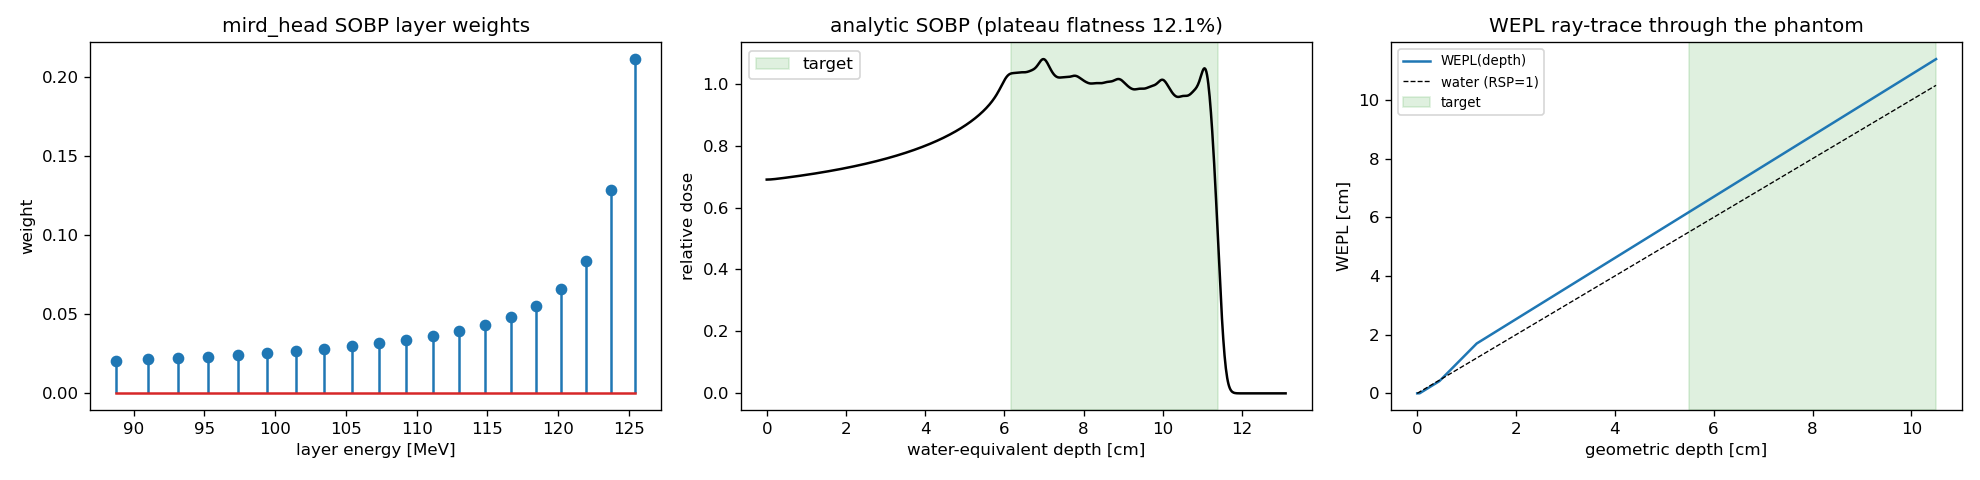
\includegraphics[width=\linewidth]{wepl_design.png}
\caption{WEPL field design for the MIRD head (\texttt{sobp.py -{}-from-run}).
\textbf{Left:} the Abel flattening weights (Eq.~\eqref{eq:wi}), heaviest on the
distal layer. \textbf{Centre:} the resulting analytic SOBP, flat across the target
in water-equivalent depth. \textbf{Right:} the WEPL ray-trace along the central
axis (Eq.~\eqref{eq:wepl}) -- the curve rises above the water diagonal, with the
kink in the first ${\sim}\SI{1.2}{cm}$ where the beam crosses scalp then skull
bone, so the geometric target window $[\SI{5.5}{},\SI{10.5}{}]\,\si{cm}$ maps to
$[\SI{6.2}{},\SI{11.4}{}]\,\si{cm}$ WEPL. This shift is the bone offset the design
absorbs.}
\label{fig:wepl}
\end{figure}

%\paragraph{Limits.} The ray-trace is one-dimensional (central axis); off-axis rays
%of the lateral disk cross slightly different skull thickness, so plateau
%uniformity over the target \emph{box} (not just the axis) is the real test
%(Sec.~\ref{sec:verify}). WEPL corrects the mean range shift but not the extra
%straggling and multiple-scattering broadening at the bone interface; if the
%verified plateau is not flat enough, the recourse is the non-negative
%least-squares weights of Sec.~\ref{sec:weights} fit to Geant4-simulated peaks.


\subsection{The phantom}
\label{sec:phantom}
\texttt{ptcryspg4} provides three phantoms, in increasing order of realism. All
share the same beam axis ($z$) and the same target-box dose normalisation; they
differ in shape and in how many materials they contain.

\paragraph{Cylinder.} A single homogeneous cylinder with its axis
along the beam. 
%The standard material is brain tissue (\texttt{G4\_BRAIN\_ICRP}) in a
%cylinder \SI{16}{cm} across and \SI{16}{cm} long --- a simple stand-in for a head,
%chosen so the isotope yields can be checked against the published numbers of Parodi
%et al.\ (2008)~\cite{parodi2008comparison}. The material is selectable: soft tissue,
%PMMA (carbon-rich), and water (which gives an almost pure-$\Ox{15}$ source) are also
%available. The carbon and oxygen content sets the mix of isotopes; the
%$\Ox{15}/\Cl{11}$ ratio is computed directly from the simulation.

\paragraph{Uniform head.} A head-shaped ellipsoid (about \SI{17}{cm} and
\SI{20}{cm} across, \SI{14}{cm} along the beam) filled with a single material, brain
tissue by default. 
%It keeps the homogeneous, clean-ground-truth character of the
%cylinder but adds the realistic outer shape, so the beam now traverses a varying
%thickness of material across its cross-section.

\paragraph{MIRD head.} A layered, anatomically realistic head built from three
nested ellipsoids: a soft-tissue scalp (\texttt{G4\_TISSUE\_SOFT\_ICRP}), a
cortical-bone skull (\texttt{G4\_BONE\_CORTICAL\_ICRP}), and a brain-tissue core
(\texttt{G4\_BRAIN\_ICRP}). This is the heterogeneous case: the dense bone layer
shifts the proton range, so the SOBP field has to be designed through the actual
scalp/skull/brain path (in water-equivalent depth) to land the dose plateau on the
target. It is the realistic counterpart to the homogeneous phantoms above.

\subsection{The physics}
\label{sec:physics}
The physics list is \texttt{QGSP\_BIC\_HP}, a hadronic list suited to proton-induced
isotope production, with electromagnetic physics and radioactive decay switched on\footnote{Geant4's isotope-production cross sections are not
as finely tuned as those of FLUKA or dedicated data-driven models, so the absolute yields carry
some bias. The same bias applies to every detector, so it cancels in a ranking; the source
files can be regenerated from a better production map.}.

\subsection{How an emitter is recorded}
\label{sec:production}
As a proton slows down it occasionally undergoes a nuclear reaction with a carbon or
oxygen nucleus, for example $\Ox{16}(p,pn)\Ox{15}$ or $\Cl{12}(p,pn)\Cl{11}$. The
leftover nucleus, created essentially at rest, is sometimes one of the positron
emitters in Table~\ref{tab:iso}. It later decays, the positron is transported over
its short range, and it annihilates. For each emitter, two points are recorded:
\begin{itemize}[nosep]
\item the \textbf{production point} --- where the emitter was made (the truth map of
where the beam created activity);
\item the \textbf{annihilation point} --- where the two \SI{511}{keV} photons are born
(the source a detector would see).
\end{itemize}
The distance between the two is the positron range for that event, so the file already
carries the resolution floor that the positron range imposes.

An emitter stays put between production and decay, so its annihilation point is fixed
by geometry alone, and its timing is supplied later by the handoff
(Sec.~\ref{sec:handoff}). (For completeness: the prompt de-excitation $\gamma$ of
$\Cl{10}$ and $\Ox{14}$, and secondary neutrons, are not tracked here --- small
omissions, noted in Sec.~\ref{sec:caveats}.)

\begin{table}[h]
\centering
\caption{The positron emitters, with half-lives and the energy that governs the
positron range. A \SI{100}{\percent} $\bplus$ branch is assumed in the handoff.}
\label{tab:iso}
\begin{tabular}{lccl}
\toprule
Isotope & $T_{1/2}$ & $\bplus$ endpoint (MeV) & Main production channel \\
\midrule
$\Ox{15}$ & \SI{122}{s}   & 1.74 & $\Ox{16}(p,pn)\Ox{15}$ \\
$\Cl{11}$ & \SI{1223}{s}  & 0.96 & $\Cl{12}(p,pn)\Cl{11}$ \\
$\Nt{13}$ & \SI{598}{s}   & 1.19 & on O / N \\
$\Cl{10}$ & \SI{19.3}{s}  & 1.91 & prompt $\gamma$ \SI{718}{keV} \\
$\Ox{14}$ & \SI{70.6}{s}  & 1.81 & prompt $\gamma$ \\
\bottomrule
\end{tabular}
\end{table}

\subsection{Setting the absolute scale}
\label{sec:norm}
The number of simulated protons is arbitrary, so on its own the emitter count has
no absolute meaning. To fix the scale, the dose deposited in a target box
inside the phantom is also scored. The ratio of the two --- emitters per unit dose ---
gives the production for a clinical dose. The standard scale is 1 Gy in the target:
from the simulated dose, the number of protons needed to deliver it
($N_p(\SI{1}{Gy})$) is computed, and the production is scaled accordingly. This is the bridge from
``some simulated protons'' to ``the absolute number of emitters for a 1 Gy
treatment'', and it provides the $P_j$ that Eq.~\eqref{eq:nmeas} consumes.

\section{Step 2 --- the handoff (how many decays are measured)}
\label{sec:handoff}

The proton run gives the number of emitters \emph{produced}. A scanner measures
fewer, because it starts after the beam and acquires for a finite time. The handoff
applies Eq.~\eqref{eq:nmeas} from Sec.~\ref{sec:kinetics} to turn the produced count
$P_j$ into the measured count $N_j$, for a chosen timing.

\paragraph{The operating point.}
This study is in-room: a full-ring scanner in the treatment room images the
patient shortly after irradiation. The baseline timing is
$t_{\mathrm{irr}}=\SI{60}{s}$, $t_{\mathrm{del}}=\SI{120}{s}$,
$t_{\mathrm{meas}}=\SI{1200}{s}$. The delay $t_{\mathrm{del}}$ is the key knob:
\SI{120}{s} is about the fastest realistic in-room delay, and longer delays are
explored by varying it. A more conservative offline point
($t_{\mathrm{del}}=\SI{300}{s}$, $t_{\mathrm{meas}}=\SI{1800}{s}$) is also provided as
a variant. As Fig.~\ref{fig:activity} shows, the short in-room delay keeps $\Ox{15}$
abundant and dominant.

\paragraph{What the handoff writes.}
The handoff writes the budget: $N_j$ per isotope, for the chosen dose and timing. It
uses no random numbers. The statistical spread of a real measurement (each count
fluctuates Poisson around $N_j$) is added later, by the downstream study, which draws
repeated Poisson realisations of the budget to estimate how precisely the range can be
recovered. The random draws live downstream, so the source side is reproducible.

\section{Using the pipeline}
\label{sec:using}

Design the beam, run the transport, compute the budget, and freeze the result as a
scenario:
\begin{verbatim}
  python3 field_design/sobp.py --mu 0.025      # design the cylinder SOBP layers
  ./proton_transport cylinder_sobp.mac         # Geant4 run -> data/runs/<tag>/
  python3 decay_sampling/budget.py data/runs/<tag>   # -> sampling_budget_inroom.csv
  python3 tools/snapshot_scenario.py cylinder_sobp_1e7   # freeze into the scenarios repo
\end{verbatim}
Full build and run instructions are in \texttt{CLAUDE.md}; the file columns are in
\texttt{common/SCHEMA.md}. A frozen run is checked with
\texttt{analysis\_transport/validate\_transport.py} (Fig.~\ref{fig:source}) and against
the Parodi 2008 yields with \texttt{analysis\_transport/parodi\_cross\_check.py}.

\section{What to keep in mind}
\label{sec:caveats}

\begin{itemize}[nosep]
\item \textbf{The phantom is homogeneous.} This means that there is no spatial $\Ox{15}/\Cl{11}$ split and no biological
washout. 
\item \textbf{Absolute yields carry a Geant4 bias.} The cross sections are not finely
tuned, so treat absolute counts as indicative. 
\item \textbf{The positron range sets a resolution floor}, largest for $\Ox{15}$. 
\end{itemize}

\bibliographystyle{unsrt}
\bibliography{biblio}

\end{document}
